\documentclass[12pt,a4paper]{article}

% ── packages ──────────────────────────────────────────────────────────────────
\usepackage[T1]{fontenc}
\usepackage[utf8]{inputenc}
\usepackage{lmodern}
\usepackage[margin=2.5cm]{geometry}
\usepackage{booktabs}
\usepackage{tabularx}
\usepackage{longtable}
\usepackage{array}
\usepackage{multirow}
\usepackage{amsmath}
\usepackage{amssymb}
\usepackage{hyperref}
\usepackage{xcolor}
\usepackage{graphicx}
\usepackage{caption}
\usepackage{setspace}
\usepackage{parskip}
\usepackage{enumitem}
\usepackage{fancyhdr}
\usepackage{titlesec}
\usepackage{microtype}

% ── colours ───────────────────────────────────────────────────────────────────
\definecolor{snbblue}{HTML}{1F6FB2}
\definecolor{charcoal}{HTML}{2C2C2C}
\definecolor{amber}{HTML}{E07B00}
\definecolor{purple}{HTML}{6A0DAD}
\definecolor{lightgray}{HTML}{F5F5F5}
\definecolor{midgray}{HTML}{888888}

% ── hyperref ──────────────────────────────────────────────────────────────────
\hypersetup{
  colorlinks = true,
  linkcolor  = snbblue,
  urlcolor   = snbblue,
  citecolor  = snbblue,
  pdftitle   = {SNB Monetary Policy: Instruments and Variables},
  pdfauthor  = {SNB\_MoPo project},
}

% ── headers ───────────────────────────────────────────────────────────────────
\pagestyle{fancy}
\fancyhf{}
\rhead{\textcolor{midgray}{\small SNB\_MoPo project}}
\lhead{\textcolor{midgray}{\small SNB Monetary Policy: Instruments and Variables}}
\rfoot{\textcolor{midgray}{\small \thepage}}
\renewcommand{\headrulewidth}{0.4pt}

% ── section formatting ────────────────────────────────────────────────────────
\titleformat{\section}{\large\bfseries\color{charcoal}}{}{0em}{}[\titlerule]
\titleformat{\subsection}{\normalsize\bfseries\color{snbblue}}{}{0em}{}
\titleformat{\subsubsection}{\normalsize\itshape\color{charcoal}}{}{0em}{}

% ── custom column types ───────────────────────────────────────────────────────
\newcolumntype{L}[1]{>{\raggedright\arraybackslash}p{#1}}
\newcolumntype{C}[1]{>{\centering\arraybackslash}p{#1}}
\newcolumntype{R}[1]{>{\raggedleft\arraybackslash}p{#1}}

% ─────────────────────────────────────────────────────────────────────────────
\begin{document}
% ─────────────────────────────────────────────────────────────────────────────

\begin{center}
  {\LARGE\bfseries SNB Monetary Policy}\\[0.4em]
  {\large Instruments, Variables, and Data}\\[1.2em]
  {\normalsize SNB\_MoPo project \quad|\quad
   \href{https://github.com/ThomasNellen/SNB_MoPo}{github.com/ThomasNellen/SNB\_MoPo}}\\[0.3em]
  {\small\textcolor{midgray}{Data vintage: April 2026}}
\end{center}

\vspace{0.5em}
\hrule height 1pt
\vspace{1.5em}

% ─────────────────────────────────────────────────────────────────────────────
\section{The SNB's Operational Framework}
% ─────────────────────────────────────────────────────────────────────────────

The Swiss National Bank (SNB) implements monetary policy through a
\textbf{tiered sight-deposit system} combined with a short-term interest-rate
target.  Since June 2019 the operational target is the \textbf{SNB policy rate}
(\texttt{LZ}), which replaces the earlier three-month CHF LIBOR target range.
The policy rate is applied to the bulk of sight deposits held by banks and other
eligible institutions at the SNB.

\subsection{Sight Deposits and the Tiering Mechanism}

Banks and certain other financial institutions hold \emph{sight deposits}
(overnight balances) at the SNB.  The SNB remunerates these deposits at
rates that depend on whether a given institution's balance exceeds an
individually calculated \emph{exemption threshold}:

\begin{itemize}[leftmargin=1.5em, itemsep=2pt]
  \item \textbf{Up to the threshold} (\texttt{ZIGBL}): since September 2022 equal
    to the policy rate.  During the negative-rate era (January 2015 to
    June 2022) this tranche was exempt from the negative rate and remunerated
    at 0\%.
  \item \textbf{Above the threshold} (\texttt{ZIG}): the charge rate applicable
    to the portion exceeding the threshold.  Since June 2022 it equals the
    policy rate; before that it equalled $-0.75$\%.
  \item \textbf{Threshold factor} (\texttt{FREI}): a multiplier applied to each
    institution's minimum reserve requirement to determine the individual
    exemption threshold.  A higher multiplier means more of a bank's deposits
    are shielded from the negative rate.  It was set at 20 from the introduction
    of the tiered system in January 2015 until October 2019, then raised
    repeatedly.
\end{itemize}

The tiering was introduced in January 2015 alongside the removal of the
EUR/CHF floor and the cut of the policy rate (then: LIBOR target midpoint) to
$-0.75$\%.  Its purpose was to avoid crushing bank profitability by allowing a
meaningful portion of reserves to be exempt from negative remuneration.  After
the SNB exited negative rates in June 2022 the distinction between \texttt{ZIGBL}
and \texttt{ZIG} effectively disappeared (both equal the policy rate), but the
legal framework remains in place.

\subsection{From LIBOR Target to Policy Rate}

\begin{itemize}[leftmargin=1.5em, itemsep=2pt]
  \item \textbf{Before June 2019}: the SNB announced a target range for the
    three-month CHF LIBOR.  The effective policy rate is approximated by the
    rate on sight deposits above the threshold (\texttt{ZIG}), which equalled
    $-0.75$\% throughout this period.
  \item \textbf{From 13 June 2019}: the SNB formally adopted the
    \textbf{SNB policy rate} (\texttt{LZ}) as its main operational target.
    The policy rate replaces the LIBOR midpoint and is directly applied to
    sight-deposit remuneration.
\end{itemize}

\subsection{SARON as the Market Rate}

The \textbf{Swiss Average Rate Overnight} (SARON) is the overnight reference
rate for the CHF money market, computed by SIX as the volume-weighted average
of all transactions and binding quotes in the Swiss franc repo market during
the trading day.  It replaced CHF LIBOR as the standard risk-free reference
rate in 2022.

Under normal operating conditions SARON tracks the SNB policy rate closely,
typically printing a few basis points \emph{below} the policy rate because
banks find it marginally cheaper to transact in the repo market than to hold
excess balances at the SNB.  Wide deviations between SARON and the policy rate
signal stress in the short-term money market.

% ─────────────────────────────────────────────────────────────────────────────
\section{Policy Decisions}
% ─────────────────────────────────────────────────────────────────────────────

The SNB Governing Board meets quarterly (typically in March, June, September,
and December) for a \emph{monetary policy assessment}.  Rate decisions are
announced on the \textbf{Thursday} of the assessment week and take effect on the
\textbf{following Friday} (the implementation date).

\medskip
\noindent Three types of events are distinguished in the dataset:

\begin{center}
\begin{tabular}{llL{7cm}}
  \toprule
  Event type & Symbol & Description \\
  \midrule
  \texttt{rate\_change} & --- & Change in ZIG / LZ (the main policy rate) \\
  \texttt{rate\_intro}  & --- & Formal introduction of the LZ policy rate
                                 (13 June 2019) \\
  \texttt{frei\_change} & --- & Change in the threshold factor (FREI) \\
  \bottomrule
\end{tabular}
\end{center}

\medskip
\noindent Announcement and implementation dates are recorded separately, allowing
event-study regressions to distinguish the \emph{announcement effect} from any
additional \emph{implementation-day effect} on SARON.

% ─────────────────────────────────────────────────────────────────────────────
\section{Liquidity Absorption (Quantitative Tightening)}
% ─────────────────────────────────────────────────────────────────────────────

After the SNB lifted rates to positive territory in June 2022, the large stock
of excess sight deposits---accumulated through FX interventions---threatened to
push SARON below the policy rate.  The SNB therefore reactivated and expanded
two market-based \textbf{liquidity-absorption} instruments: SNB Bills and
reverse repos.

\subsection{SNB Bills (Schatzwechsel)}

SNB Bills are short-term, zero-coupon securities \emph{issued by the SNB}
and purchased by eligible counterparties (banks, securities dealers, and similar
institutions).  The purchase transfers CHF from the banking system to the SNB,
thereby shrinking excess reserves for the bill's tenor.

\subsubsection{Auction mechanics}

\begin{itemize}[leftmargin=1.5em, itemsep=2pt]
  \item \textbf{Frequency}: every Thursday.
  \item \textbf{Subscription window}: 11:00--11:30 CET/CEST.
  \item \textbf{Auction type}: Variable Rate, American allotment (VR,\,A)---each
    accepted bidder pays their own submitted price.
  \item \textbf{Settlement}: payment four calendar days after the auction
    (\textit{T}\,+\,4); redemption at face value (CHF 1\,000\,000 per bill) on
    the maturity date.
  \item \textbf{Maturities}: two tranches per week, always including a
    \textbf{28-day} tranche.  The second tranche rotates across
    84\,d\,$\to$\,168\,d\,$\to$\,84\,d\,$\to$\,336\,d in a roughly four-week
    cycle, giving four standard tenors in all.
  \item \textbf{Issuance type}: \texttt{N}\,=\,new ISIN (new series);
    \texttt{A}\,=\,tap (additional tranche under an existing ISIN).
\end{itemize}

\subsubsection{History and scale}

SNB Bills were first issued in October 2008 as an ad-hoc sterilisation tool
during the global financial crisis.  They fell dormant during the negative-rate
era (2015--2022) and were reactivated in August 2022 alongside the return to
positive rates.  Since then outstanding volume has grown substantially:

\begin{center}
\begin{tabular}{lrr}
  \toprule
  Period & Peak outstanding & Source \\
  \midrule
  2008--2012 (first episode) & CHF $\approx$25\,bn   & snbbipo (ES) \\
  2022--2026 (current episode) & CHF $\approx$99\,bn & snbbipo (ES) \\
  \bottomrule
\end{tabular}
\end{center}

\subsubsection{Pricing}

The marginal yield in SNB Bill auctions is consistently a few basis points
\emph{below} the policy rate (typically $-5$ to $-10$\,bp), reflecting the
opportunity cost to banks of committing liquidity for up to twelve months
relative to maintaining overnight balances at the SNB.  Yields on longer
tranches (168\,d, 336\,d) lie slightly above the 28-day yield, forming a
mildly upward-sloping short-end curve.

\subsection{Reverse Repos (Liquidity-Absorbing Repos)}

In a \textbf{reverse repo} from the SNB's perspective, the SNB \emph{sells}
CHF-denominated securities (typically Confederation bonds or agency paper) to
a counterparty under an agreement to repurchase them after the term.  The
counterparty pays CHF now and receives securities; the SNB receives CHF and
holds the repurchase obligation.  Net effect: CHF is absorbed from the banking
system for the repo term.

\noindent This should not be confused with the SNB's \emph{liquidity-providing}
repos, in which the SNB \emph{buys} securities from banks (a repo from the
bank's perspective).

\subsubsection{Auction mechanics}

\begin{itemize}[leftmargin=1.5em, itemsep=2pt]
  \item \textbf{Frequency}: every bank working day.
  \item \textbf{Subscription window}: 09:00--09:10 CET/CEST on normal days;
    delayed to 10:30--10:40 on monetary policy assessment days
    (approximately quarterly).
  \item \textbf{Standard term}: 7 calendar days (occasionally 14 days
    around holidays or policy meetings).
  \item \textbf{Settlement}: payment T+2; redemption T+2+term.
  \item \textbf{Auction type}: Variable Rate, American allotment (VR,\,A).
  \item \textbf{Holiday closures}: no auction on Swiss public holidays; gaps
    also around Easter, Ascension, and Whitsun.
\end{itemize}

\subsubsection{Data availability}

The SNB publishes only a forward-looking auction schedule (updated quarterly,
PDF format).  \emph{No transaction-level results database exists in the public
domain.}  Monthly outstanding balances are available from the SNB balance sheet
via the \texttt{snbbipo} cube (series \texttt{VRGSF}).

% ─────────────────────────────────────────────────────────────────────────────
\section{Variable Definitions}
% ─────────────────────────────────────────────────────────────────────────────

\subsection{Daily Rate Series (\texttt{snbgwdzid} cube)}

All rates in per cent per annum; daily frequency.

\begin{longtable}{L{2.2cm} L{4.5cm} L{2.5cm} L{5.3cm}}
  \toprule
  \textbf{Code} & \textbf{Name} & \textbf{Available from} & \textbf{Notes} \\
  \midrule
  \endhead
  \bottomrule
  \endfoot
  \texttt{LZ}    & SNB policy rate
                 & 13 Jun 2019
                 & Replaced the three-month CHF LIBOR target as the main
                   operational rate.  Before this date, ZIG ($-0.75$\%)
                   proxies the effective policy rate. \\[4pt]
  \texttt{ZIG}   & Sight-deposit rate above threshold
                 & Jan 2015
                 & Rate applied to deposits exceeding the exemption threshold.
                   Equals LZ since Jun 2022; was $-0.75$\% throughout the
                   negative-rate era. \\[4pt]
  \texttt{ZIGBL} & Sight-deposit rate up to threshold
                 & Sep 2022 (recorded)
                 & Rate applied to deposits within the exemption threshold.
                   Was effectively 0\% from Jan 2015 to Jun 2022 (exemption
                   from negative charge); back-filled with 0 in our dataset.
                   Equals LZ since Jun 2022. \\[4pt]
  \texttt{FREI}  & Threshold factor
                 & Nov 2019 (recorded)
                 & Multiplier applied to minimum reserve requirements to
                   compute the individual exemption threshold.  Was 20 from
                   Jan 2015 to Oct 2019; back-filled with 20 in our dataset. \\[4pt]
  \texttt{ZIABP} & Discount (basis points)
                 & Sep 2022
                 & Spread between ZIGBL and ZIG in basis points.
                   Currently 0 (rates unified since Jun 2022). \\[4pt]
  \texttt{SARON} & Swiss Average Rate Overnight
                 & Aug 2009
                 & SIX overnight fixing; volume-weighted average of repo
                   transactions and binding quotes.  Main CHF risk-free
                   reference rate since the discontinuation of CHF LIBOR
                   (Dec 2021). \\[4pt]
  \texttt{ENG}   & Special rate (Sondersatz)
                 & May 2004
                 & Rate applied to certain intraday and emergency facilities;
                   not directly relevant to the tiering system. \\
\end{longtable}

\subsection{Policy Decisions Table (\texttt{policy\_decisions.csv})}

One row per SNB decision event; 24 events from Dec 2014 to Mar 2025.

\begin{center}
\begin{tabular}{L{3.2cm} L{3.2cm} L{7cm}}
  \toprule
  \textbf{Column} & \textbf{Type} & \textbf{Description} \\
  \midrule
  \texttt{announce\_date}  & date    & Thursday of the monetary policy assessment \\
  \texttt{implement\_date} & date    & Friday following the assessment (effective date) \\
  \texttt{event\_type}     & string  & \texttt{rate\_change}, \texttt{rate\_intro},
                                       or \texttt{frei\_change} \\
  \texttt{ZIG\_new}        & float   & New ZIG rate (\%), if changed \\
  \texttt{LZ\_new}         & float   & New policy rate LZ (\%), if applicable \\
  \texttt{FREI\_new}       & float   & New threshold factor, if changed \\
  \texttt{label}           & string  & Short descriptive label for the event \\
  \bottomrule
\end{tabular}
\end{center}

\subsection{SNB Bills Auction Data (\texttt{snb\_bills\_auctions.csv})}

One row per ISIN per auction; 393 rows covering August 2022 to April 2026.

\begin{center}
\begin{tabular}{L{3.8cm} L{2.5cm} L{7.5cm}}
  \toprule
  \textbf{Column} & \textbf{Type} & \textbf{Description} \\
  \midrule
  \texttt{auction\_date}         & date    & Date of the auction (Thursday) \\
  \texttt{isin}                  & string  & ISIN of the security (CH\ldots) \\
  \texttt{denomination\_chf}     & integer & Face value per bill (CHF 1\,000\,000) \\
  \texttt{issuance\_type}        & string  & \texttt{N}\,=\,new ISIN; \texttt{A}\,=\,tap \\
  \texttt{term\_days}            & integer & Exact calendar days from payment to redemption \\
  \texttt{payment\_date}         & date    & Settlement date (T+4) \\
  \texttt{redemption\_date}      & date    & Maturity date \\
  \texttt{auction\_type}         & string  & Always ``VR,\,A'' (variable rate, American) \\
  \texttt{marginal\_price\_pct}  & float   & Marginal accepted price as \% of face value \\
  \texttt{yield\_pct}            & float   & Yield at the marginal price, per cent p.a. \\
  \texttt{bids\_chf\_mn}         & float   & Total bids submitted (CHF mn); published end of month \\
  \texttt{allotment\_chf\_mn}    & float   & Total allotment to market (CHF mn) \\
  \texttt{allot\_issuer\_chf\_mn}& float   & SNB's own retention (CHF mn) \\
  \texttt{outstanding\_chf\_mn}  & float   & Outstanding volume for this ISIN after auction (CHF mn) \\
  \texttt{term\_bucket}          & string  & Rounded tenor: \texttt{7d}, \texttt{28d},
                                             \texttt{84d}, \texttt{168d}, \texttt{336d} \\
  \bottomrule
\end{tabular}
\end{center}

\noindent\textbf{Note on publication timing:} the SNB publishes the marginal price
on the first bank working day after the auction at 18:00.  Bids, allotment, and
outstanding volumes are published on the last bank working day of the
\emph{following} month; rows for the most recent auctions therefore show
\texttt{NaN} for those columns until the publication date.

\subsection{Weekly Bills Aggregation (\texttt{snb\_bills\_weekly.csv})}

One row per auction date; allotment summed by term bucket.

\begin{center}
\begin{tabular}{L{4.2cm} L{2.5cm} L{7.1cm}}
  \toprule
  \textbf{Column} & \textbf{Type} & \textbf{Description} \\
  \midrule
  \texttt{auction\_date}          & date  & Auction Thursday \\
  \texttt{7d}                     & float & Allotment in the 7-day tranche (CHF mn) \\
  \texttt{28d}                    & float & Allotment in the 28-day tranche (CHF mn) \\
  \texttt{84d}                    & float & Allotment in the 84-day tranche (CHF mn) \\
  \texttt{168d}                   & float & Allotment in the 168-day tranche (CHF mn) \\
  \texttt{336d}                   & float & Allotment in the 336-day tranche (CHF mn) \\
  \texttt{total\_allotment\_chf\_mn} & float & Sum across all tranches (CHF mn) \\
  \bottomrule
\end{tabular}
\end{center}

\subsection{Monthly Balance Sheet (\texttt{snb\_balance\_sheet\_monthly.csv})}

Monthly end-of-period balance sheet positions from the \texttt{snbbipo} cube,
CHF millions.

\begin{center}
\begin{tabular}{L{4.4cm} L{2.3cm} L{2.4cm} L{4.7cm}}
  \toprule
  \textbf{Column} & \textbf{SNB code} & \textbf{From} & \textbf{Description} \\
  \midrule
  \texttt{snb\_bills\_outstanding\_ chf\_mn}      & \texttt{ES}    & Oct 2008 &
    Outstanding SNB Bills (liability side).  Sum of all live ISINs. \\[4pt]
  \texttt{reverse\_repo\_liabilities\_chf\_mn}    & \texttt{VRGSF} & Apr 1998 &
    Reverse repo liabilities in CHF: SNB's obligation to repurchase
    securities sold under repo.  Measures cumulative liquidity absorbed
    through reverse repos. \\[4pt]
  \texttt{repo\_claims\_chf\_mn}                  & \texttt{FRGSF} & Apr 1998 &
    Repo claims in CHF: SNB's claims from liquidity-\emph{providing} repos
    (asset side).  Not a QT instrument. \\[4pt]
  \texttt{sight\_deposits\_chf\_mn}               & \texttt{N}     & Dec 1996 &
    Sight deposits of domestic banks (liability side).  Main stock of
    excess reserves in the banking system. \\[4pt]
  \texttt{total\_assets\_chf\_mn}                 & \texttt{T0}    & Dec 1996 &
    Total assets of the SNB balance sheet. \\[4pt]
  \texttt{banknotes\_chf\_mn}                     & \texttt{UA}    & Dec 1996 &
    Banknotes in circulation. \\[4pt]
  \texttt{total\_liq\_absorption\_chf\_mn}        & derived        & Oct 2008 &
    $\texttt{ES} + \texttt{VRGSF}$: total liquidity absorbed through
    bills and reverse repos combined. \\
  \bottomrule
\end{tabular}
\end{center}

% ─────────────────────────────────────────────────────────────────────────────
\section{Data Sources and Reproducibility}
% ─────────────────────────────────────────────────────────────────────────────

\begin{center}
\begin{tabular}{L{3.5cm} L{10.5cm}}
  \toprule
  \textbf{Source} & \textbf{URL / reference} \\
  \midrule
  SNB Data Portal & \url{https://data.snb.ch} \\
  Daily rates cube & \url{https://data.snb.ch/api/cube/snbgwdzid/data/csv/en} \\
  Balance sheet cube & \url{https://data.snb.ch/api/cube/snbbipo/data/csv/en} \\
  SNB Bills results & \url{https://www.snb.ch/public/bills/snbBillsResults.pdf} \\
  Repo auction schedule & \url{https://www.snb.ch/public/repos/repoAuctionSchedule.pdf} \\
  Bills calendar & \url{https://www.snb.ch/public/bills/snbBillsCalendar.pdf} \\
  Policy decisions & Compiled manually from SNB press releases \\
  \bottomrule
\end{tabular}
\end{center}

\medskip
\noindent All data are downloaded and processed by two scripts in the
\texttt{code/} directory:

\begin{itemize}[leftmargin=1.5em, itemsep=2pt]
  \item \texttt{snb\_mopo\_analysis.py}: daily rates, policy decisions, and the
    tiered-system figure.
  \item \texttt{snb\_qt\_analysis.py}: SNB Bills auction data and monthly
    balance sheet positions.
\end{itemize}

Running either script from the project root reproduces the processed datasets
in \texttt{input/processed/} from scratch.  Raw downloads are cached in
\texttt{input/raw/} (gitignored) and only re-downloaded if absent.

% ─────────────────────────────────────────────────────────────────────────────
\section{Figure: Tiered Sight-Deposit Remuneration and SARON}
% ─────────────────────────────────────────────────────────────────────────────

\begin{figure}[h!]
  \centering
  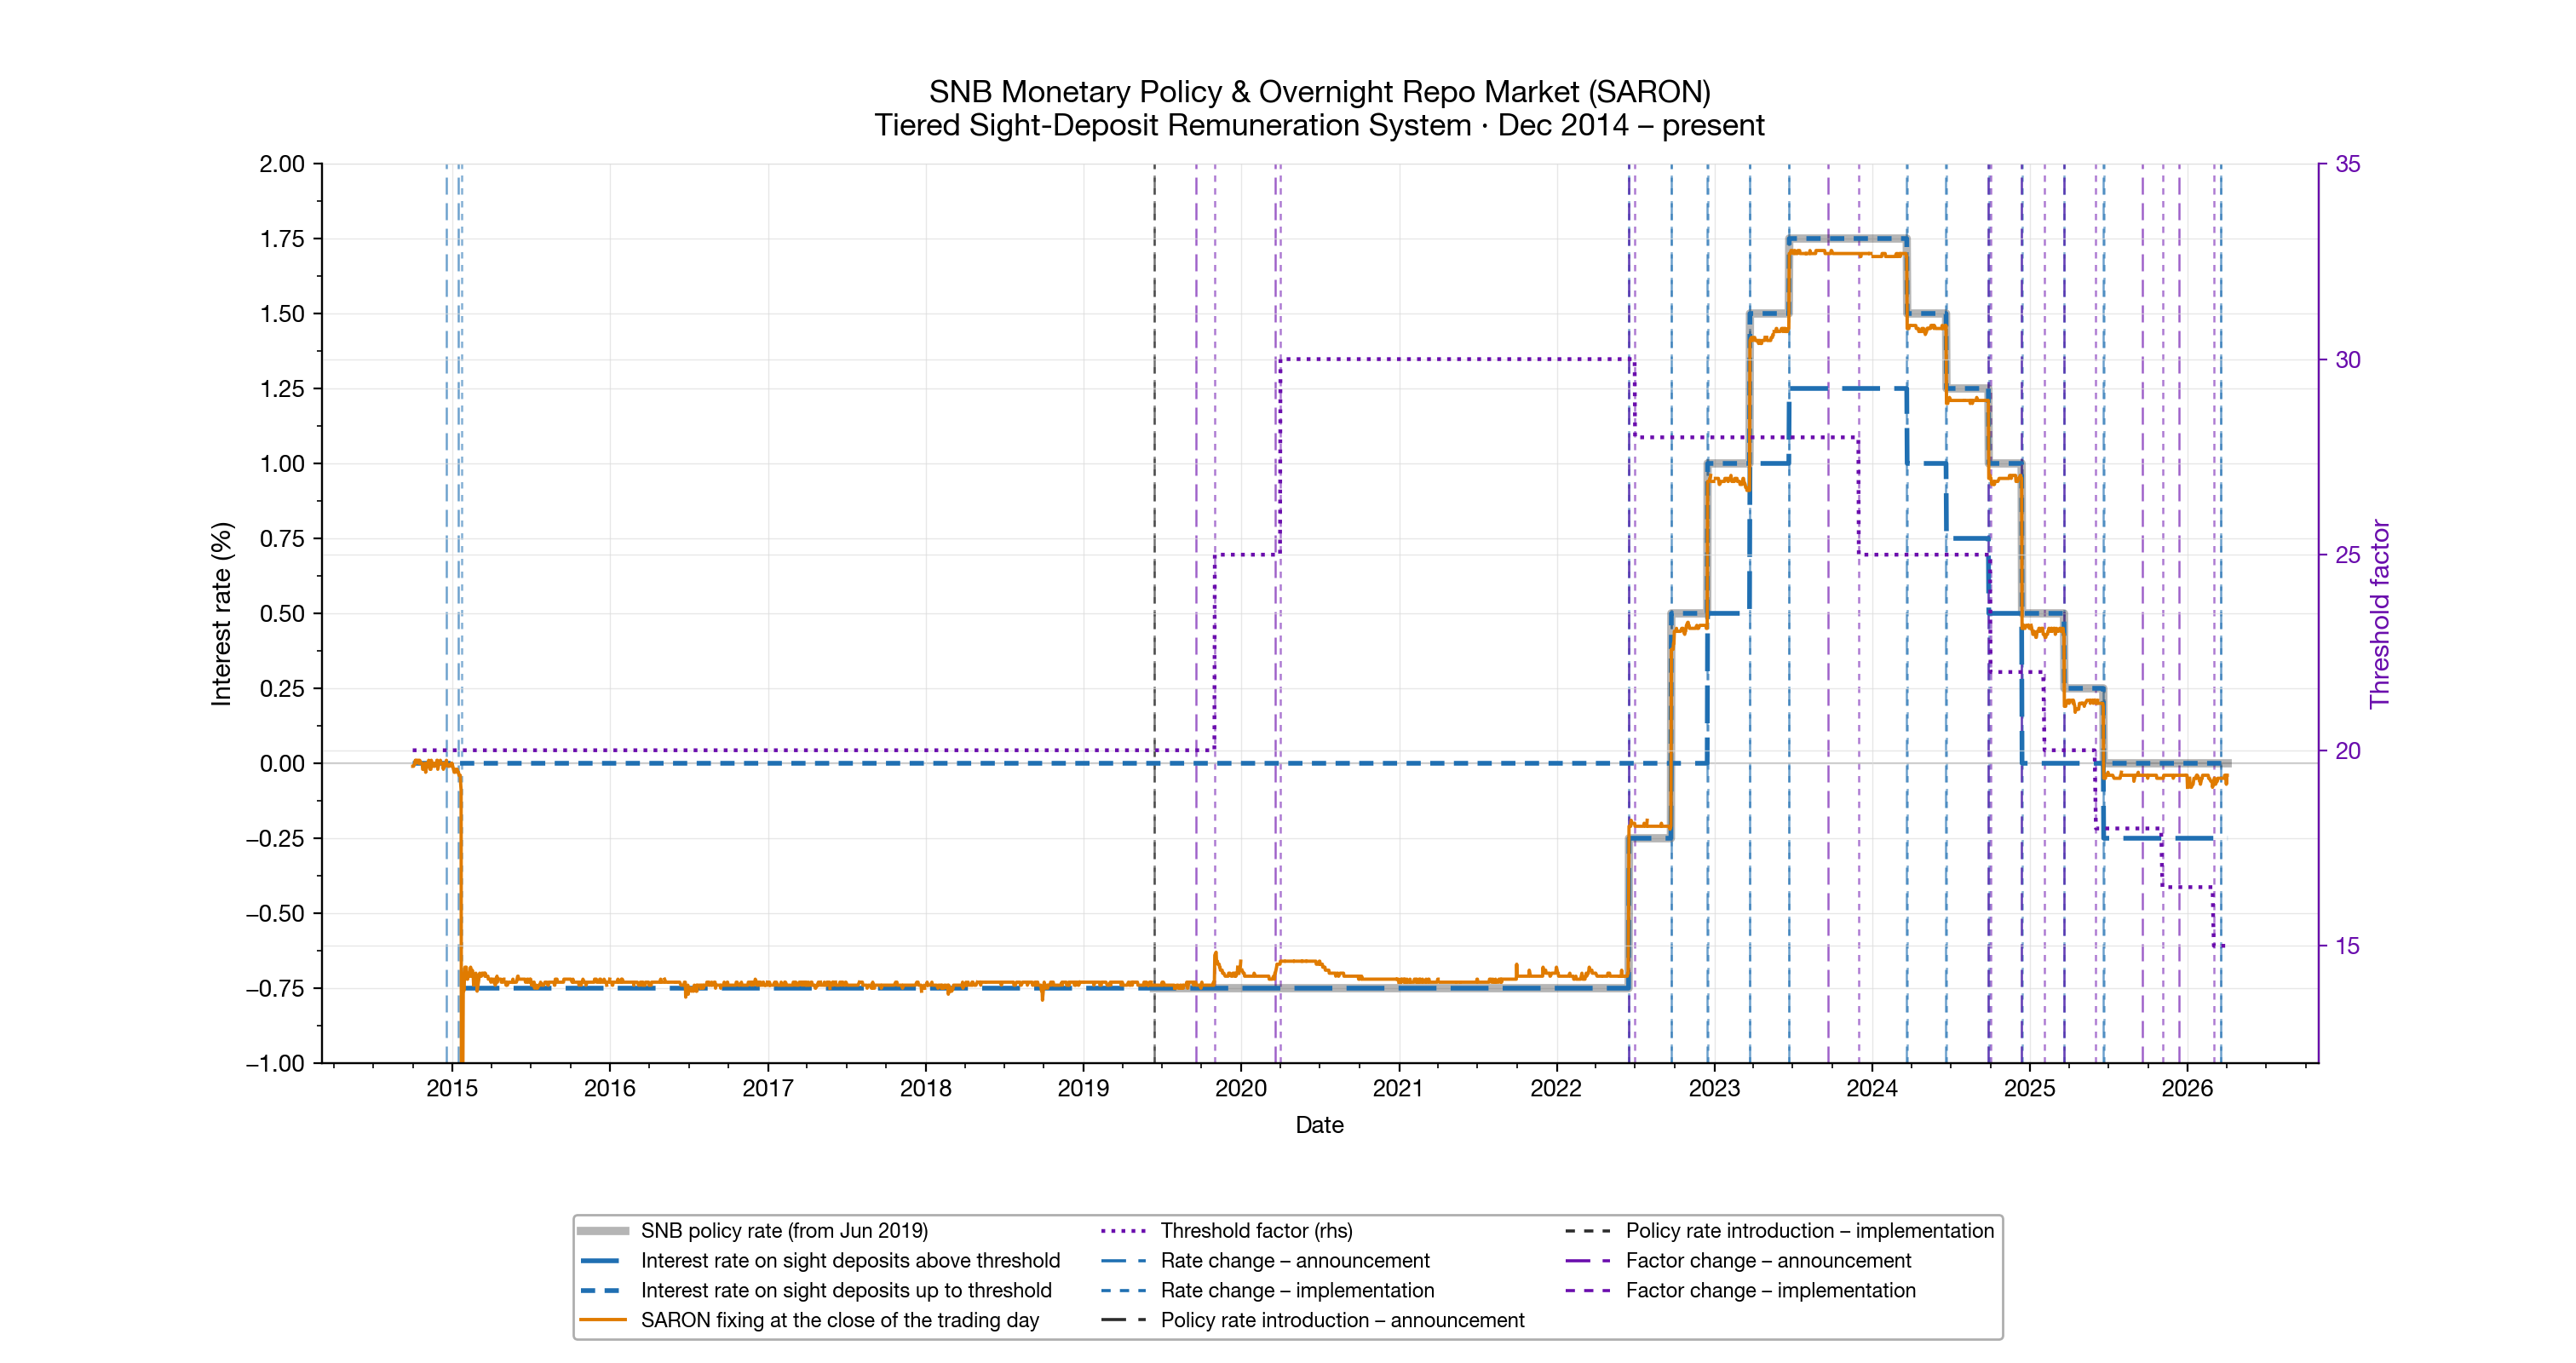
\includegraphics[width=\linewidth]{Figure_MoPo_SARON.png}
  \caption{SNB policy rates, sight-deposit remuneration tiers, threshold
    factor (right axis), and SARON since December 2014.
    Vertical dashed lines mark SNB announcement dates (long dashes) and
    implementation dates (short dashes), coloured by the type of change:
    \textcolor{snbblue}{steel blue} for rate changes,
    \textcolor{charcoal}{charcoal} for the policy-rate introduction, and
    \textcolor{purple}{purple} for threshold-factor changes.
    Source: SNB Data Portal (\texttt{snbgwdzid}); own computation.}
  \label{fig:tiered_system}
\end{figure}

% ─────────────────────────────────────────────────────────────────────────────
\end{document}
